\documentclass{article}
\iffalse
This file is protected by Copyright. Please refer to the COPYRIGHT file
distributed with this source distribution.

This file is part of OpenCPI <http://www.opencpi.org>

OpenCPI is free software: you can redistribute it and/or modify it under the
terms of the GNU Lesser General Public License as published by the Free Software
Foundation, either version 3 of the License, or (at your option) any later
version.

OpenCPI is distributed in the hope that it will be useful, but WITHOUT ANY
WARRANTY; without even the implied warranty of MERCHANTABILITY or FITNESS FOR A
PARTICULAR PURPOSE. See the GNU Lesser General Public License for more details.

You should have received a copy of the GNU Lesser General Public License along
with this program. If not, see <http://www.gnu.org/licenses/>.
\fi

\author{} % Force author to be blank
%----------------------------------------------------------------------------------------
% Paper size, orientation and margins
%----------------------------------------------------------------------------------------
\usepackage{geometry}
\geometry{
	letterpaper,			% paper type
	portrait,				% text direction
	left=.75in,				% left margin
	top=.75in,				% top margin
	right=.75in,			% right margin
	bottom=.75in			% bottom margin
 }
%----------------------------------------------------------------------------------------
% Header/Footer
%----------------------------------------------------------------------------------------
\usepackage{fancyhdr} \pagestyle{fancy} % required for fancy headers
\usepackage{multirow}
\usepackage{longtable}
\renewcommand{\headrulewidth}{0.5pt}
\renewcommand{\footrulewidth}{0.5pt}
\rhead{\small{ANGRYVIPER Team}}
%----------------------------------------------------------------------------------------
% Appendix packages
%----------------------------------------------------------------------------------------
\usepackage[toc,page]{appendix}
%----------------------------------------------------------------------------------------
% Defined Commands & Renamed Commands
%----------------------------------------------------------------------------------------
\renewcommand{\contentsname}{Table of Contents}
\renewcommand{\listfigurename}{List of Figures}
\renewcommand{\listtablename}{List of Tables}
\newcommand{\todo}[1]{\textcolor{red}{TODO: #1}\PackageWarning{TODO:}{#1}} % To do notes
\newcommand{\code}[1]{\texttt{#1}} % For inline code snippet or command line
%----------------------------------------------------------------------------------------
% Various pacakges
%----------------------------------------------------------------------------------------
\usepackage{hyperref} % for linking urls and lists
\usepackage{graphicx} % for including pictures by file
\usepackage{listings} % for coding language styles
\usepackage{rotating} % for sideways table
\usepackage{pifont}   % for sideways table
\usepackage{pdflscape} % for landscape view
%----------------------------------------------------------------------------------------
% Table packages
%----------------------------------------------------------------------------------------
\usepackage{longtable} % for long possibly multi-page tables
\usepackage{tabularx} % c=center,l=left,r=right,X=fill
\usepackage{float}
\floatstyle{plaintop}
\usepackage[tableposition=top]{caption}
\newcolumntype{P}[1]{>{\centering\arraybackslash}p{#1}}
\newcolumntype{M}[1]{>{\centering\arraybackslash}m{#1}}
%----------------------------------------------------------------------------------------
% Block Diagram / FSM Drawings
%----------------------------------------------------------------------------------------
\usepackage{tikz}
\usetikzlibrary{shapes,arrows,fit,positioning}
\usetikzlibrary{automata} % used for the fsm
\usetikzlibrary{calc} % For duplicating clients
\usepgfmodule{oo} % To define a client box
%----------------------------------------------------------------------------------------
% Colors Used
%----------------------------------------------------------------------------------------
\usepackage{colortbl}
\definecolor{blue}{rgb}{.7,.8,.9}
\definecolor{ceruleanblue}{rgb}{0.16, 0.32, 0.75}
\definecolor{drkgreen}{rgb}{0,0.6,0}
\definecolor{deepmagenta}{rgb}{0.8, 0.0, 0.8}
\definecolor{cyan}{rgb}{0.0,0.6,0.6}
\definecolor{maroon}{rgb}{0.5,0,0}
%----------------------------------------------------------------------------------------
% Update the docTitle and docVersion per document
%----------------------------------------------------------------------------------------
\def\docTitle{Platform Data Sheet}
\def\docVersion{1.5}
%----------------------------------------------------------------------------------------
\date{Version \docVersion} % Force date to be blank and override date with version
\title{\docTitle}
\lhead{\small{\docTitle}}

\def\comp{ml605}
\edef\ecomp{ml605}
\def\Comp{ML605 Platform}
\graphicspath{ {figures/} }

\begin{document}

\section*{Zipper Deprecation Notice:}
\textbf{Beginning with OpenCPI Version 1.5, support for Lime Microsystems' Zipper card is now deprecated.}


\section*{Summary - \Comp}
\begin{tabular}{|c|M{13.5cm}|}
	\hline
	\rowcolor{blue}
	                  & \\
	\hline
	Name              & \comp \\
	\hline
	Worker Type       & Platform \\
	\hline
	Version           & v\docVersion \\
	\hline
	Release Date      & 4/2019 \\
	\hline
	Library & ocpi.assets.platforms \\
	\hline
	Workers & \comp.hdl \\
	\hline
\end{tabular}

\section*{Functionality}
\begin{flushleft}
	The ML605 platform worker provides an interface between a PCIe-connected processor and the Virtex-6 FPGA on the ML605 board. It makes connections over a PCIe bus for OpenCPI control and data planes. It also provides a 200 MHz clock source for the timebase port and a 125 MHz clock source for the control plane.
\end{flushleft}

\section*{Worker Implementation Details}
\begin{flushleft}
	The ML605 platform worker instantiates version 1.7 of the Xilinx LogiCORE IP Virtex-6 FPGA Integrated Block for PCI Express. This Integrated Block is compatible with the PCI Express Card Electromechanical v2.0 and PCI Industrial Computer Manufacturers Group 3.4 specifications. The 4-lane Gen1/Gen2 implementation is used. The intended clock source frequency is 250 MHz. For detailed information of the LogiCORE functionality and usage, refer to Xilinx UG715 and Xilinx DS517. Figure \ref{fig:blockdiagram} diagrams the intra-worker functionality of the ml605 platform worker.\medskip

	\begin{figure}[h]
		\centering\captionsetup{type=figure}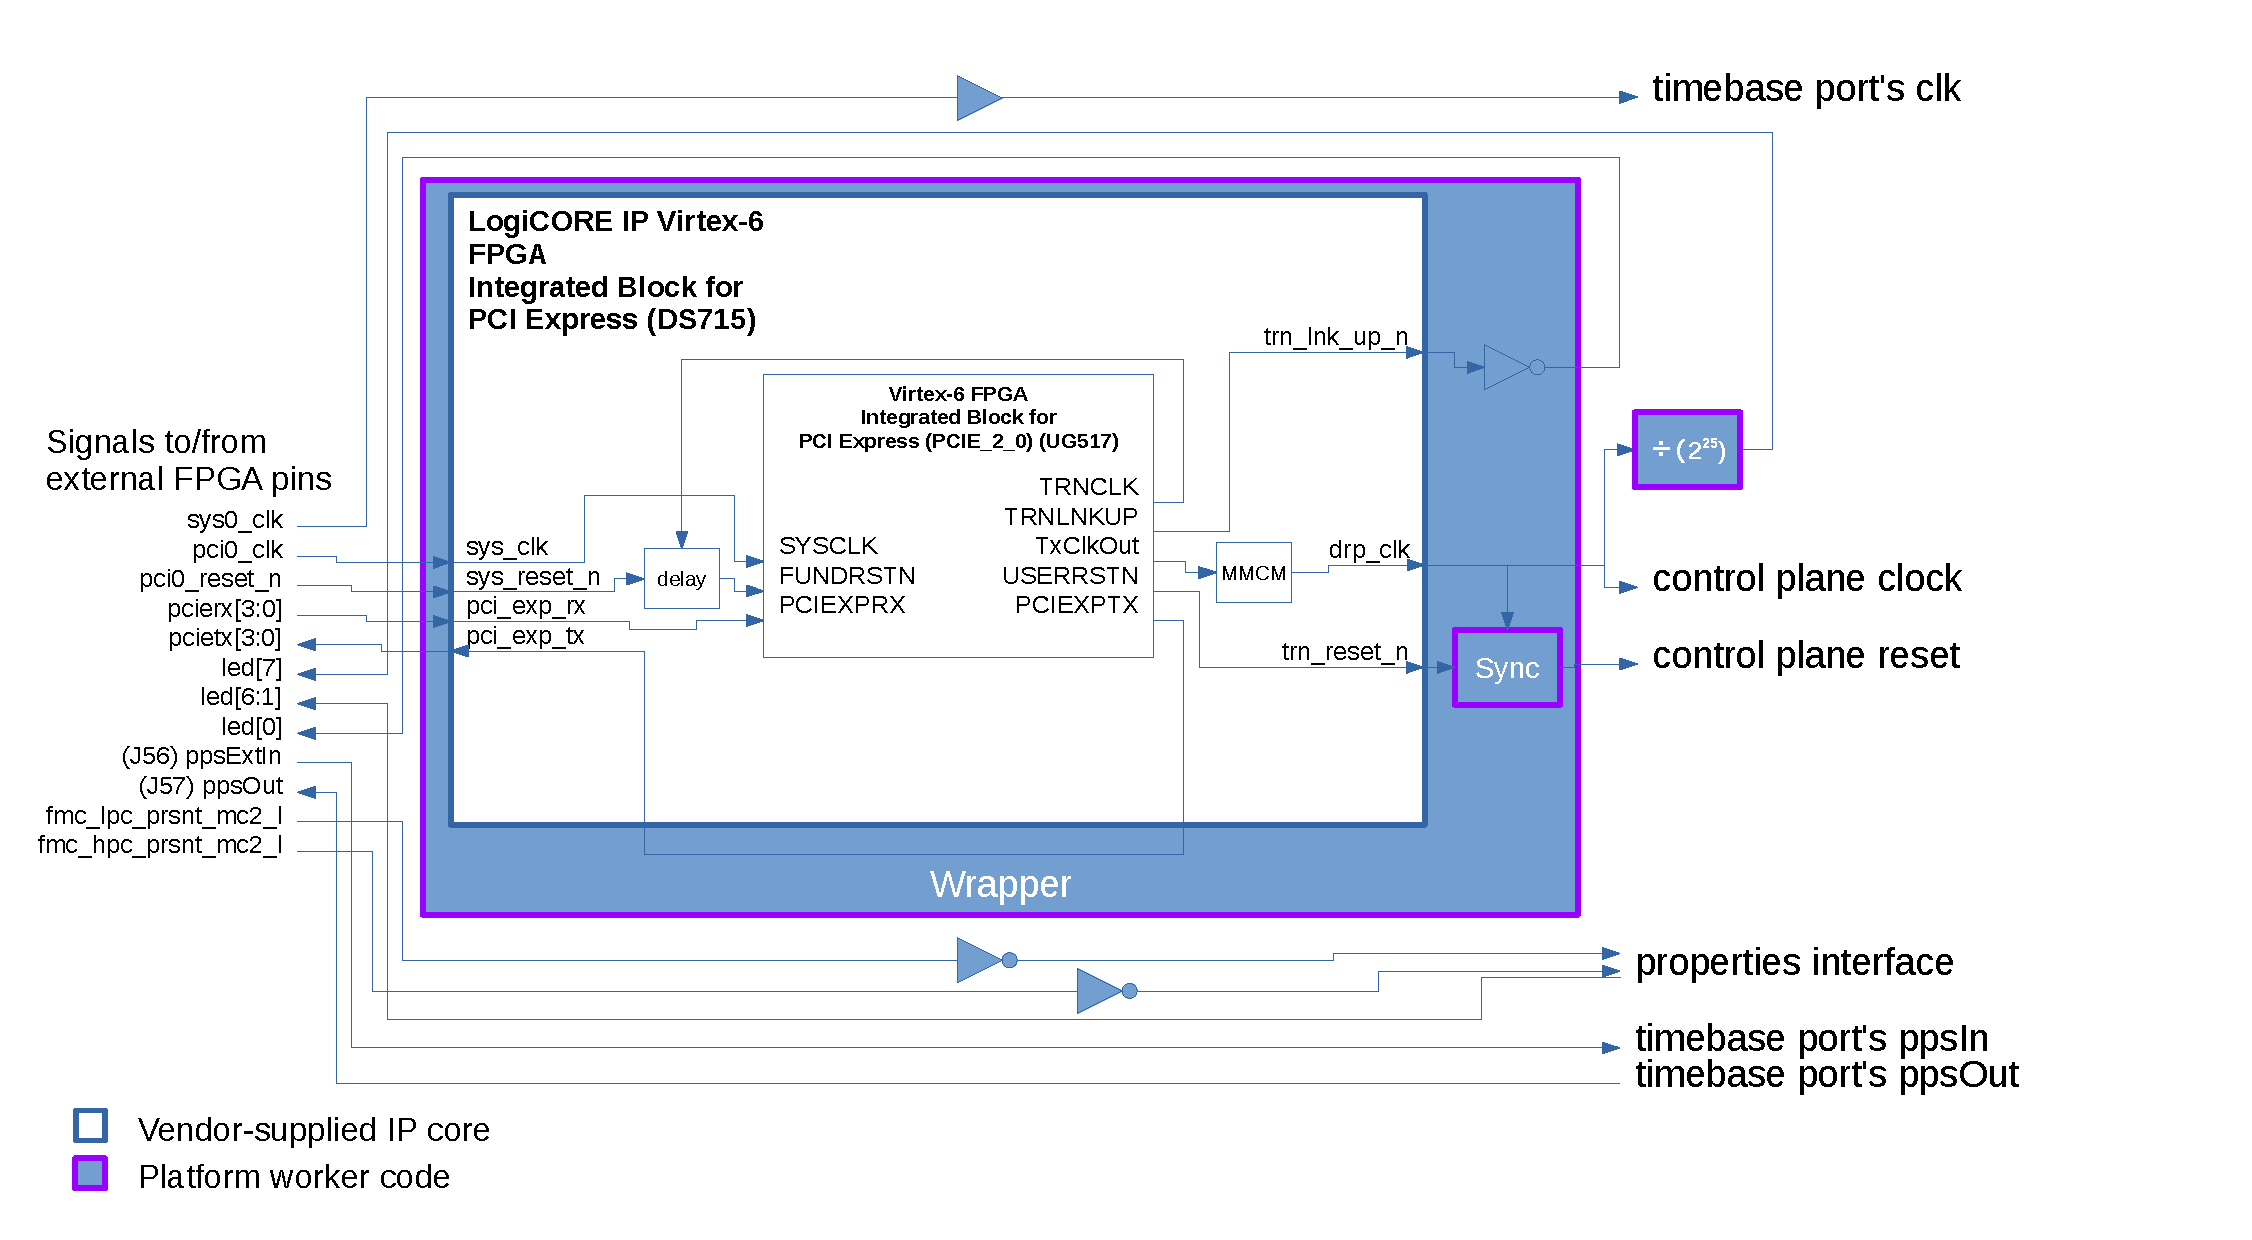
\includegraphics[scale=0.5]{ml605_platform_worker_block_diagram}
		\captionof{figure}{ml605 Functional Diagram}
		\label{fig:blockdiagram}
	\end{figure}
\end{flushleft}
\pagebreak

\section*{Theory}
Because there are no data processing algorithms implemented in this worker, no corresponding data processing theory is relevant herein.

\section*{Block Diagrams}
\subsection*{Top level}
\makeatletter
\newcommand{\gettikzxy}[3]{%
  \tikz@scan@one@point\pgfutil@firstofone#1\relax
  \edef#2{\the\pgf@x}%
  \edef#3{\the\pgf@y}%
}
\makeatother
\pgfooclass{clientbox}{ % This is the class clientbox
    \method clientbox() { % The clientbox
    }
    \method apply(#1,#2,#3,#4) { % Causes the clientbox to be shown at coordinate (#1,#2) and named #3
        \node[rectangle,draw=white,fill=white] at (#1,#2) (#3) {#4};
    }
}
\pgfoonew \myclient=new clientbox()
\begin{center}
  \begin{tikzpicture}[% List of styles applied to all, to override specify on a case-by-case
      every node/.style={
        align=center,      % use this so that the "\\" for line break works
        minimum size=2cm,  % creates space above and below text in rectangle
        minimum width=4cm
      },
      every edge/.style={draw,thick}
    ]
    \node[rectangle,ultra thick,draw=black,fill=blue](R2){\Comp};
    \node[rectangle,draw=white,fill=white,minimum size=1.0cm](R5)[below= of R2]{timebase};
    \node[rectangle,draw=white,fill=white](placeholder)[above= of R2]{};
    \path[->]
    (R2)edge []  node [] {} (R5)
    (R5)edge []  node [] {} (R2)
    ;
    \gettikzxy{(placeholder)}{\rx}{\ry}
    \myclient.apply(\rx - 40,\ry,C1,\\ metadata);
    \path[<->]($(R2.north) + (-40 pt,0)$) edge [] node [] {} (C1);
    \myclient.apply(-\rx + 40,\ry,C1, ``pcie'' \\ unoc control/data plane );
    \path[<->]($(R2.north) + (40 pt,0)$) edge [] node [] {} (C1);

  \end{tikzpicture}
\end{center}

\subsection*{State Machines}
No state machines exist within the platform worker outside of those within the PCIe LogiCORE IP block. It is not intended for users of LogiCORE IP blocks to understand their inner functionality.

\newpage
\section*{Source Dependencies}
\begin{itemize}
	\item
assets/hdl/platforms/ml605/ml605.vhd
	\item
assets/hdl/platforms/ml605/pci\_ml605.v
	\item
assets/hdl/platforms/ml605/ml605\_pkg.vhd
	\item
assets/hdl/primitives/virtex6/xilinx\_v6\_pcie\_wrapper.v
	\item
assets/hdl/primitives/pcie\_4243\_trn\_v6\_gtx\_x4\_250/gtx\_drp\_chanalign\_fix\_3752\_v6.v
	\item
assets/hdl/primitives/pcie\_4243\_trn\_v6\_gtx\_x4\_250/gtx\_rx\_valid\_filter\_v6.v
	\item
assets/hdl/primitives/pcie\_4243\_trn\_v6\_gtx\_x4\_250/gtx\_tx\_sync\_rate\_v6.v
	\item
assets/hdl/primitives/pcie\_4243\_trn\_v6\_gtx\_x4\_250/gtx\_wrapper\_v6.v
	\item
assets/hdl/primitives/pcie\_4243\_trn\_v6\_gtx\_x4\_250/Makefile
	\item
assets/hdl/primitives/pcie\_4243\_trn\_v6\_gtx\_x4\_250/pcie\_2\_0\_v6.v
	\item
assets/hdl/primitives/pcie\_4243\_trn\_v6\_gtx\_x4\_250/pcie\_brams\_v6.v
	\item
assets/hdl/primitives/pcie\_4243\_trn\_v6\_gtx\_x4\_250/pcie\_bram\_top\_v6.v
	\item
assets/hdl/primitives/pcie\_4243\_trn\_v6\_gtx\_x4\_250/pcie\_bram\_v6.v
	\item
assets/hdl/primitives/pcie\_4243\_trn\_v6\_gtx\_x4\_250/pcie\_clocking\_v6.v
	\item
assets/hdl/primitives/pcie\_4243\_trn\_v6\_gtx\_x4\_250/pcie\_gtx\_v6.v
	\item
assets/hdl/primitives/pcie\_4243\_trn\_v6\_gtx\_x4\_250/pcie\_pipe\_lane\_v6.v
	\item
assets/hdl/primitives/pcie\_4243\_trn\_v6\_gtx\_x4\_250/pcie\_pipe\_misc\_v6.v
	\item
assets/hdl/primitives/pcie\_4243\_trn\_v6\_gtx\_x4\_250/pcie\_pipe\_v6.v
	\item
assets/hdl/primitives/pcie\_4243\_trn\_v6\_gtx\_x4\_250/pcie\_reset\_delay\_v6.v
	\item
assets/hdl/primitives/pcie\_4243\_trn\_v6\_gtx\_x4\_250/pcie\_upconfig\_fix\_3451\_v6.v
	\item
assets/hdl/primitives/pcie\_4243\_trn\_v6\_gtx\_x4\_250/v6\_pcie\_v1\_7\_bb.v
	\item
assets/hdl/primitives/pcie\_4243\_trn\_v6\_gtx\_x4\_250/v6\_pcie\_v1\_7.v
\end{itemize}

\begin{landscape}
	\section*{Component Spec Properties}
	\begin{scriptsize}
		\begin{tabular}{|p{3cm}|p{1.5cm}|c|c|c|p{1.5cm}|p{1cm}|p{6cm}|}
			\hline
			\rowcolor{blue}
			Name               & Type   & SequenceLength & ArrayDimensions & Accessibility      & Valid Range & Default & Usage                                                                         \\
			\hline
			\verb+platform+    & String & 31             & -               & Parameter & Standard & - & Name of this platform                                                     \\
			\hline
			\verb+sdp_width+   & UChar  & -              & -               & Parameter & Standard & 1 & Width of data plane in DWORDS \newline \textbf{(SDP is NOT implemented by the ml605)}   \\
			\hline
			\verb+UUID+        & ULong  & -              & 16              & Readable           & Standard    & -       & UUID of this platform                                                         \\
			\hline
			\verb+oldtime+     & ULongLong & -           & -               & Padding            & Standard    & -       & N/A                                                                           \\
			\hline
			\verb+romAddr+     & UShort & -              & -               & Writable           & Standard    & -       &                                                                               \\
			\hline
			\verb+romData+     & ULong  & -              & -               & Volatile           & Standard    & -       &                                                                               \\
			\hline
			\verb+nSwitches+   & ULong  & -              & -               & Readable           & Standard    & -       & Number of switches                                                            \\
			\hline
			\verb+nLEDs+       & ULong  & -              & -               & Readable           & Standard    & -       & Number of LEDs                                                                \\
			\hline
			\verb+memories_length+ & ULong & -           & -               & Readable           & Standard    & -       &                                                                               \\
			\hline
			\verb+memories+    & ULong  & -              & 4               & Readable           & Standard    & -       & The memory regions that may be used by \\
  	                     &        &                &                 &                    &             &         & various other elements, which          \\
  	                     &        &                &                 &                    &             &         & indicates aliasing etc.               \\
                         &        &                &                 &                    &             &         & The values describing each region are: \\
                         &        &                &                 &                    &             &         & Bit 31:28 - External bus/BAR connected \\
                         &        &                &                 &                    &             &         &             to this memory (0 is none) \\
                         &        &                &                 &                    &             &         & Bit 27:14 - Offset in bus/BAR of this  \\
                         &        &                &                 &                    &             &         &             memory (4KB units)         \\
                         &        &                &                 &                    &             &         & Bit  13:0 - Size of this memory (4KB units) \\
                         &        &                &                 &                    &             &         &             units) \\
			\hline
			\verb+dna+         & ULongLong & -           & -               & Readable           & Standard    & -       & DNA (unique chip serial number) of this platform \\
			\hline
			\verb+switches+    & ULong  & -              & -               & Volatile           & Standard    & -       & Current value of any switches in the platform                                 \\
			\hline
			\verb+LEDS+        & ULong  & -              & -               & Writable, Readable & Standard    & -       & Setting of LEDs in the platform, with readback. A value of true illuminates the given LED. The indices and their corresponding LEDs are index 12: LED DS17, 11: DS18, 10: DS20, 9: DS19, 8: DS16, 7: unused, 6: DS22, 5: DS15, 4: DS13, 3: DS10, 2: DS9, 1: DS11, 0: unused. For example, writing a value of 0x1002 will illuminate only LEDs DS17 and DS11.\\
			\hline
			\verb+nSlots+      & ULong  & -              & -               & Parameter & Standard & 0 & Number of slots available for cards, which indicates the usable length of the slotCardIsPresent array property. \\
			\hline
			\verb+slotNames+   & String & 32             & -               & Parameter & Standard & ``'' & A string which is intended to include comma-separated names of the slots available for cards. The inter-comma position of each name corresponds to the same index of the slotCardIsPresent array property. \\
			\hline
			\verb+pci_device_id+ & Enum & -              & -               & Parameter & unknown, ml605, alst4, alst4x & unknown & PCI Device ID for PCI devices. This is essentially the ``registry'' of PCI device IDs. New platforms can use ``unknown'' before they are registered. \\
			\hline
			\verb+slotCardIsPresent+ & Bool & -          & 64              & Volatile           & Standard    & -       & An array of booleans, where each index contains an indication whether a card is physically present in the given index's slot. For a description of a given index's slot, see the corresponding comma-separated string contents in the slotName property. Note that only the first min(nSlots,64) of the 64 indices contain pertinent information. \\
			\hline

		\end{tabular}
	\end{scriptsize}
	\section*{Worker Properties}
	\begin{scriptsize}
		\begin{tabular}{|p{1.5cm}|p{2.5cm}|p{1cm}|c|c|c|p{2cm}|p{2cm}|p{3cm}|}
			\hline
			\rowcolor{blue}
			Type     & Name                      & Type  & SequenceLength & ArrayDimensions & Accessibility       & Valid Range & Default & Usage                                      \\
			\hline
			SpecProperty & \verb+platform+       & String & 31            & -               & Parameter & Standard & ml605 & Name of this platform               \\
			\hline
			SpecProperty & \verb+nSlots+         & ULong  & -             & -               & Parameter & Standard & 2 & Number of slots available for cards, which indicates the usable length of the slotCardIsPresent array property. \\
			\hline
			SpecProperty & \verb+slotNames+      & String & 32            & -               & Parameter & Standard & fmc\_lpc,fmc\_hpc & A string which is intended to include comma-separated names of the slots available for cards. The inter-comma position of each name corresponds to the same index of the slotCardIsPresent array property. \\
			\hline
			SpecProperty & \verb+pci_device_id+ & Enum & -              & -               & Parameter & unknown, ml605, alst4, alst4x & ml605 & PCI Device ID for PCI devices. This is essentially the ``registry'' of PCI device IDs. New platforms can use ``unknown'' before they are registered. \\
			\hline
			Property & \verb+pciId+              & UShort & -             & -               & Volatile            & Standard    & -       &                                  \\
			\hline
			Property & \verb+unocDropCount+      & UChar & -              & -               & Volatile            & Standard    & -       & Invalid packets collected at uNOC terminator \\
			\hline
		\end{tabular}
	\end{scriptsize}

	\section*{Component Ports}
	No ports are implemented for the given component specification.

	\section*{Worker Interfaces}
	\begin{scriptsize}
		\begin{tabular}{|M{2cm}|M{2cm}|M{1.5cm}|M{1.5cm}|M{14.5cm}|}
			\hline
			\rowcolor{blue}
			Type       & Name & Master & Count & Usage                  \\
			\hline
			metadata   & -    & true   & -     & Access to container metadata via the platform worker. All platform workers must provide this port. \\
			\hline
			timebase   & -    & true   & -     & Providing a timebase for the time service. All platform workers must provide this port. \\
			\hline
			unoc       & pcie & true   & -     & This platform worker provides a control/data plane called ``pcie''. \\
			\hline
		\end{tabular}
	\end{scriptsize}

\end{landscape}
\pagebreak

\section*{Platform Devices}
The following table enumerates the device workers that are included in the base platform configuration. The parameter values specified restrict allowed implementations. Note that the worker signals listed are only those who are unconnected on the platform or whose platform signal name differ from the worker signal name. Note that device workers allowed by cards are not included in this list. \\ \newline
\begin{tabular}{|M{3cm}|M{3.5cm}|M{3cm}|M{3cm}|M{3cm}|}
	\hline
	\rowcolor{blue}
	Name                       & Property Name    & Property Value              & Worker Signal & Platform Signal         \\
	\hline
	time\_server               & frequency        & 200*10\textsuperscript{6}   &               &                         \\
	\hline
	flash &   &   &  &  \\
	\hline
\end{tabular}

\section*{Signals}
Note that this signal table does not include signals that may be provided by slots. \\
\begin{tabular}{|c|c|c|c|p{8cm}|}
	\hline
	\rowcolor{blue}
	Name           & Type   & Differential & Width & Description                                          \\
	\hline
	sys0\_clk      & Input  & true         & 1     & 200 MHz clock which is sent to the timebase port.    \\
	\hline
	sys1\_clk      & Input  & true         & 1     & GBE clock (unused).                                  \\
	\hline
	pci0\_clk      & Input  & true         & 1     & 250 MHz clock which is sent to the LogiCORE PCIE block. \\
	\hline
	pci0\_reset\_n & Input  & false        & 1     & PCIe reset.                                          \\
	\hline
	pcie\_rx       & Input  & true         & 4     & PCIe RX.                                             \\
	\hline
	pcie\_tx       & Output & true         & 4     & PCIe TX.                                             \\
	\hline
	led            & Output & false        & 13    & led[12:8] drive the LEDs labelled DS17, DS18, DS20, DS19, and DS16 in the schematic, respectively. led[7:0] drive the LEDs labelled DS21, DS22, DS14, DS15, DS10, DS9, DS11, DS12 in the schematic, respectively. led[12:8] and led[6:1] are driven by the 12:8 and 6:1 indices of the LEDS property. led[7] is driven by the PCIE-generated control plane clock divided by 2\textsuperscript{25} and led[0] is driven by the PCIE link up indicator. A high voltage on these signals illuminates their respective LEDs.\\
	\hline
	ppsExtIn       & Input  & false        & 1     & This signal is driven by external hardware connected to the ML605 board's J56 SMA connector. The purpose of this signal is to provide a PPS clock source to the worker connected to the timebase port. Note that said worker may or may not use this signal. \\
	\hline
	ppsOut         & Output & false        & 1     & The worker connected to the timebase port drives this signal, which is connected to the J57 SMA connector. The purpose of this signal is for said worker to output the PPS signal it produces. Note that said worker may use a variety of clock sources to produce its PPS, not necessarily the corresponding ppsExtIn signal. \\
	\hline
	fmc\_lpc\_prsnt\_mc2\_l & Input & false & 1    & Connected to the PRSNTn signal of the FMC LPC slot. (Device workers may not ingest the FMC HPC PRSNTn signal). This active-low signal provides FMC LPC mezzanine card presence indication to index 0 of the slotCardIsPresent property.         \\
	\hline
	fmc\_hpc\_prsnt\_mc2\_l & Input & false & 1    & Connected to the PRSNTn signal of the FMC HPC slot. (Device workers may not ingest the FMC HPC PRSNTn signal). This active-low signal provides FMC HPC mezzanine card presence indication to index 1 of the slotCardIsPresent property. \\
	\hline
\end{tabular}
\pagebreak
\section*{Slots}
The following table enumerates the available slots for this platform and the signals they include. Note that the signals listed are only those who are unconnected on the platform or whose platform signal name do not match the slot signal name. \\
\begin{longtable}[l]{|c|c|c|c|}
	\hline
	\rowcolor{blue}
	Name           & Type & Slot Signal & Platform Signal  \\
	\hline
	\multirow{2}{*}{FMC\_LPC} & \multirow{2}{*}{fmc\_lpc} & LA00\_P\_CC & FMC\_LPC\_LA00\_CC\_P \
	\\\cline{3-4}
	& & LA00\_P\_CC & FMC\_LPC\_LA00\_CC\_P \
	\\\cline{3-4}
	& & LA00\_N\_CC & FMC\_LPC\_LA00\_CC\_N \
	\\\cline{3-4}
	& & LA01\_P\_CC & FMC\_LPC\_LA01\_CC\_P \
	\\\cline{3-4}
	& & LA01\_N\_CC & FMC\_LPC\_LA01\_CC\_N \
	\\\cline{3-4}
	& & LA17\_P\_CC & FMC\_LPC\_LA17\_CC\_P \
	\\\cline{3-4}
	& & LA17\_N\_CC & FMC\_LPC\_LA17\_CC\_N \
	\\\cline{3-4}
	& & DP0\_C2M\_P & - \
	\\\cline{3-4}
	& & DP0\_C2M\_N & - \
	\\\cline{3-4}
	& & DP0\_M2C\_P & - \
	\\\cline{3-4}
	& & DP0\_M2C\_N & - \
	\\\cline{3-4}
	& & LA18\_P\_CC & FMC\_LPC\_LA18\_CC\_P \
	\\\cline{3-4}
	& & LA18\_N\_CC & FMC\_LPC\_LA18\_CC\_N \
	\\\cline{3-4}
	& & SCL & FMC\_LPC\_IIC\_SCL\_LS \
	\\\cline{3-4}
	& & SDA & FMC\_LPC\_IIC\_SDA\_LS \\
	\hline
	\multirow{2}{*}{FMC\_HPC} & \multirow{2}{*}{fmc\_hpc} & LA00\_P\_CC & FMC\_HPC\_LA00\_CC\_P \
	\\\cline{3-4}
	& & LA00\_N\_CC & FMC\_HPC\_LA00\_CC\_N \
	\\\cline{3-4}
	& & LA01\_P\_CC & FMC\_HPC\_LA01\_CC\_P \
	\\\cline{3-4}
	& & LA01\_N\_CC & FMC\_HPC\_LA01\_CC\_N \
	\\\cline{3-4}
	& & LA17\_P\_CC & FMC\_HPC\_LA17\_CC\_P \
	\\\cline{3-4}
	& & LA17\_N\_CC & FMC\_HPC\_LA17\_CC\_N \
	\\\cline{3-4}
	& & DP0\_C2M\_P & - \
	\\\cline{3-4}
	& & DP0\_C2M\_N & - \
	\\\cline{3-4}
	& & DP0\_M2C\_P & - \
	\\\cline{3-4}
	& & DP0\_M2C\_N & - \
	\\\cline{3-4}
	& & LA18\_P\_CC & FMC\_HPC\_LA18\_CC\_P \
	\\\cline{3-4}
	& & LA18\_N\_CC & FMC\_HPC\_LA18\_CC\_N \
	\\\cline{3-4}
  & & DP9\_M2C\_P & - \
  \\\cline{3-4}
  & & DP9\_M2C\_N & - \
  \\\cline{3-4}
  & & DP8\_M2C\_P & - \
  \\\cline{3-4}
  & & DP8\_M2C\_N & - \
  \\\cline{3-4}
  & & DP7\_M2C\_P & - \
  \\\cline{3-4}
  & & DP7\_M2C\_N & - \
  \\\cline{3-4}
  & & DP6\_M2C\_P & - \
  \\\cline{3-4}
  & & DP6\_M2C\_N & - \
  \\\cline{3-4}
  & & DP9\_C2M\_P & - \
  \\\cline{3-4}
  & & DP9\_C2M\_N & - \
  \\\cline{3-4}
  & & DP8\_C2M\_P & - \
  \\\cline{3-4}
  & & DP8\_C2M\_N & - \
  \\\cline{3-4}
  & & DP7\_C2M\_P & - \
  \\\cline{3-4}
  & & DP7\_C2M\_N & - \
  \\\cline{3-4}
  & & DP6\_C2M\_P & - \
  \\\cline{3-4}
  & & DP6\_C2M\_N & - \
  \\\cline{3-4}
  & & DP1\_M2C\_P & - \
  \\\cline{3-4}
  & & DP1\_M2C\_N & - \
  \\\cline{3-4}
  & & DP2\_M2C\_P & - \
  \\\cline{3-4}
  & & DP2\_M2C\_N & - \
  \\\cline{3-4}
  & & DP3\_M2C\_P & - \
  \\\cline{3-4}
  & & DP3\_M2C\_N & - \
  \\\cline{3-4}
  & & DP4\_M2C\_P & - \
  \\\cline{3-4}
  & & DP4\_M2C\_N & - \
  \\\cline{3-4}
  & & DP5\_M2C\_P & - \
  \\\cline{3-4}
  & & DP5\_M2C\_N & - \
  \\\cline{3-4}
  & & DP1\_C2M\_P & - \
  \\\cline{3-4}
  & & DP1\_C2M\_N & - \
  \\\cline{3-4}
  & & DP2\_C2M\_P & - \
  \\\cline{3-4}
  & & DP2\_C2M\_N & - \
  \\\cline{3-4}
  & & DP3\_C2M\_P & - \
  \\\cline{3-4}
  & & DP3\_C2M\_N & - \
  \\\cline{3-4}
  & & DP4\_C2M\_P & - \
  \\\cline{3-4}
  & & DP4\_C2M\_N & - \
  \\\cline{3-4}
  & & DP5\_C2M\_P & - \
  \\\cline{3-4}
  & & DP5\_C2M\_N & - \
  \\\cline{3-4}
  & & HA00\_P\_CC & HA00\_CC\_P \
  \\\cline{3-4}
  & & HA00\_N\_CC & HA00\_CC\_N \
  \\\cline{3-4}
  & & HA01\_P\_CC & HA01\_CC\_P \
  \\\cline{3-4}
  & & HA01\_N\_CC & HA01\_CC\_N \
  \\\cline{3-4}
  & & HA17\_P\_CC & HA17\_CC\_P \
  \\\cline{3-4}
  & & HA17\_N\_CC & HA17\_CC\_N \
  \\\cline{3-4}
  & & HB00\_P\_CC & HB00\_CC\_P \
  \\\cline{3-4}
  & & HB00\_N\_CC & HB00\_CC\_N \
  \\\cline{3-4}
  & & HB06\_P\_CC & HB06\_CC\_P \
  \\\cline{3-4}
  & & HB06\_N\_CC & HB06\_CC\_N \
  \\\cline{3-4}
  & & HB17\_P\_CC & HB17\_CC\_P \
  \\\cline{3-4}
  & & HB17\_N\_CC & HB17\_CC\_N \
  \\\cline{3-4}
  & & PG\_M2C & PG\_M2C\_LS \
  \\\cline{3-4}
	& & SCL & IIC\_SCL\_MAIN\_LS \
	\\\cline{3-4}
	& & SDA & IIC\_SDA\_MAIN\_LS \\
	\hline
\end{longtable}

\newpage
\section*{Platform Configurations}
Below is a sample set of supported platform configurations which  highlight the device workers included in the platform configuration versus card/slots. For a complete list of supported platform configurations, refer to the ml605 directory. \\

\begin{tabular}{|c|c|c|c|}
	\hline
	\rowcolor{blue}
	Name & Platform Configuration Workers & Card & Slot \\
	\hline
	\multirow{2}{*}{base} &ml605 & - & - \\ &time\_server & - & - \\
	\hline
	\multirow{2}{*}{ml605\_flash} &ml605 & - & - \\ &time\_server & -
	& - \\ &flash & - & - \\
	\hline
	\multirow{5}{*}{ml605\_zipper\_fmc\_lpc\_rx\_tx}&
	ml605 & - & - \\ &time\_server & - & - \\
	&lime\_adc & lime\_zipper\_fmc\_lpc & fmc\_lpc \\ &lime\_dac &
	lime\_zipper\_fmc\_lpc & fmc\_lpc \\ &si5351 &
	lime\_zipper\_fmc\_lpc & fmc\_lpc \\ &lime\_rx &
	lime\_zipper\_fmc\_lpc & fmc\_lpc \\ &lime\_tx &
	lime\_zipper\_fmc\_lpc & fmc\_lpc \\
	\hline
	\multirow{5}{*}{ml605\_zipper\_fmc\_lpc\_rx}&
	ml605 & - & - \\ &time\_server & - & - \\
	&lime\_adc & lime\_zipper\_fmc\_lpc & fmc\_lpc \\  &si5351 &
	lime\_zipper\_fmc\_lpc & fmc\_lpc \\ &lime\_rx &
	lime\_zipper\_fmc\_lpc & fmc\_lpc \\
	\hline
	\multirow{5}{*}{ml605\_zipper\_fmc\_lpc\_tx}&
	ml605 & - & - \\ &time\_server & - & - \\
	&lime\_dac & lime\_zipper\_fmc\_lpc & fmc\_lpc \\  &si5351 &
	lime\_zipper\_fmc\_lpc & fmc\_lpc \\ &lime\_tx &
	lime\_zipper\_fmc\_lpc & fmc\_lpc \\
	\hline
	\multirow{5}{*}{ml605\_zipper\_fmc\_hpc\_rx\_tx}&
	ml605 & - & - \\ &time\_server & - & - \\
	&lime\_adc & lime\_zipper\_fmc\_hpc & fmc\_hpc \\ &lime\_dac &
	lime\_zipper\_fmc\_hpc & fmc\_hpc \\ &si5351 &
	lime\_zipper\_fmc\_hpc & fmc\_hpc \\ &lime\_rx &
	lime\_zipper\_fmc\_hpc & fmc\_hpc \\ &lime\_tx &
	lime\_zipper\_fmc\_hpc & fmc\_hpc \\
	\hline
	\multirow{5}{*}{ml605\_zipper\_fmc\_hpc\_rx}&
	ml605 & - & - \\ &time\_server & - & - \\
	&lime\_adc & lime\_zipper\_fmc\_hpc & fmc\_hpc \\  &si5351 &
	lime\_zipper\_fmc\_hpc & fmc\_hpc \\ &lime\_rx &
	lime\_zipper\_fmc\_hpc & fmc\_hpc \\
	\hline
	\multirow{5}{*}{ml605\_zipper\_fmc\_hpc\_tx}&
	ml605 & - & - \\ &time\_server & - & - \\
	&lime\_dac & lime\_zipper\_fmc\_hpc & fmc\_hpc \\  &si5351 &
	lime\_zipper\_fmc\_hpc & fmc\_hpc \\ &lime\_tx &
	lime\_zipper\_fmc\_hpc & fmc\_hpc \\
	\hline
\end{tabular}

\newpage	
\section*{Control Timing and Signals}
There are 3 clock domains present in the ml605 platform worker: 250 MHz, 125 MHz, and 200 MHz. The worker ingests an external-to-the FPGA 250 MHz clock. This clock serves as the clock source for the LogiCORE PCIe Integrated Block within the worker. The LogiCORE block divides the 250 MHz clock down to a 125 MHz clock which is subsequently supplied to the control plane as its clock. The worker also feeds a buffered version of the external-to-the-FPGA 200 MHz clock to the timebase port. The timebase port is also supplied with a PPS from the ML605 board's J56 SMA connector. The timebase port also include a PPS output which is fed to the J57 SMA connector.

\begin{landscape}
\section*{Performance and Resource Utilization}
In the following Platform Worker Utilization tables, the Worker Build Configuration ``0'' refers to the Platform Worker itself. Named configurations refer to platform configurations (\textit{e.g.} they may include other device workers along with the Platform Worker).\\\\
\input{../../\ecomp/utilization.inc}
\end{landscape}

\section*{Test and Verification}
\begin{flushleft}
 To be detailed in a future release.
\end{flushleft}
\section*{References}
\begin{flushleft}
	\begin{itemize}
		\item[1)] Virtex-6 FPGA Integrated Block for PCI Express User Guide (DS715), \url{https://www.xilinx.com/support/documentation/user_guides/v6_pcie_ug517.pdf} \\
		\item[2)] LogiCORE IP Virtex-6 FPGA Integrated Block v1.7 for PCI Express (UG517), \url{https://www.xilinx.com/support/documentation/ip_documentation/v6_pcie_ds715.pdf}
	\end{itemize}
\end{flushleft}


\end{document}
